% !TeX program = pdflatex
\documentclass[12pt,a4paper]{article}

% -------------------- Paquetes --------------------
\usepackage[T1]{fontenc}
\usepackage[utf8]{inputenc}
\usepackage[spanish,mexico]{babel}
\usepackage{helvet}
\renewcommand{\familydefault}{\sfdefault}
\usepackage[a4paper,margin=2.5cm]{geometry}
\usepackage{graphicx}
\usepackage{float}
\usepackage{caption}
\usepackage{subcaption}
\usepackage{amsmath,amssymb}
\usepackage{xcolor}
\usepackage{listings}
\usepackage{fancyhdr}
\usepackage{setspace}
\usepackage{hyperref}

\graphicspath{{../images/}}
\setstretch{1.15}
\hypersetup{colorlinks=true,linkcolor=blue,urlcolor=blue}

\lstdefinestyle{vhdl}{
  language=VHDL,
  basicstyle=\ttfamily\small,
  keywordstyle=\color{blue!70!black}\bfseries,
  commentstyle=\color{gray!80!black},
  numbers=left,
  numberstyle=\tiny\color{gray},
  numbersep=8pt,
  frame=single,
  breaklines=true,
  showstringspaces=false,
  tabsize=2
}
\lstset{style=vhdl}

\pagestyle{fancy}
\fancyhf{}
\fancyhead[L]{Laboratorio de Diseño Lógico}
\fancyhead[R]{Práctica 1}
\fancyfoot[C]{\thepage}
\setlength{\headheight}{15pt}

\begin{document}

% -------------------- Portada --------------------
\begin{titlepage}
  \centering
  {\Large Universidad Autónoma Metropolitana\\}
  {\large Unidad Azcapotzalco\\}
  {\large División de Ciencias Básicas e Ingeniería\\[1.2cm]}
  {\large UEA 1121040\\}
  {\large Laboratorio de Diseño Lógico\\[1.5cm]}
  {\large Profesor: Eduardo Rodríguez Martínez\\[2cm]}
  {\LARGE\bfseries Práctica 1\\[0.4cm]}
  {\Large Multiplexores y decodificación de salidas\\[2cm]}
  {\large Flores Olivares Omar\\}
  {\large Matrícula: 2243038415\\}
  {\large Trimestre 26-O\\}
  {\large al2243038415@azc.uam.mx\\}
  \vfill
  {\large Noviembre de 2026}
\end{titlepage}

\tableofcontents
\newpage

% -------------------- Objetivo --------------------
\section{Objetivo}
Desarrollar circuitos digitales descritos en VHDL e implementarlos de manera modular en la tarjeta de desarrollo Altera DE2. La práctica utiliza interruptores como entradas y LEDs o displays de siete segmentos como salidas, con el propósito de relacionar las expresiones booleanas, la descripción estructural y el comportamiento esperado de los circuitos.

\section{Material y herramientas}
\begin{itemize}
  \item Tarjeta de desarrollo Altera DE2.
  \item Quartus II para describir, integrar y compilar los diseños.
  \item Lenguaje VHDL.
  \item Manual de usuario e instructivo de la tarjeta DE2 incluidos en la carpeta \texttt{Material}.
\end{itemize}

\section{Desarrollo}

\subsection{Parte 2. Multiplexor 2 a 1 de ocho bits}

\subsubsection{Descripción del ejercicio}
Se construye un multiplexor de dos entradas de ocho bits a partir de una descripción VHDL que implementa la selección de cada bit. El selector \(S\) determina cuál de los dos vectores se transmite a la salida \(M\).

Para cada posición \(i\), la función lógica es:
\[
M(i)=\overline{S}\,X(i)+S\,Y(i), \qquad i\in\{0,\ldots,7\}.
\]
Por lo tanto, cuando \(S=0\), la salida corresponde a \(X\); cuando \(S=1\), corresponde a \(Y\).

\begin{figure}[H]
  \centering
  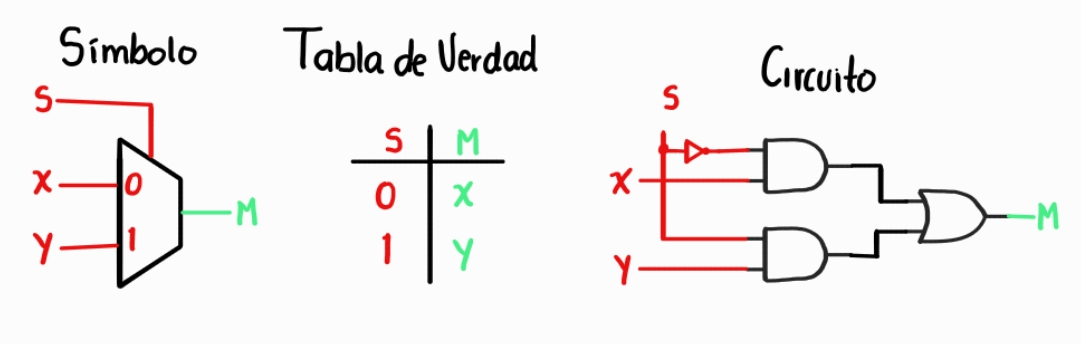
\includegraphics[width=0.55\textwidth]{figura1.jpg}
  \caption{Representación del multiplexor 2 a 1 de un bit.}
\end{figure}

\begin{figure}[H]
  \centering
  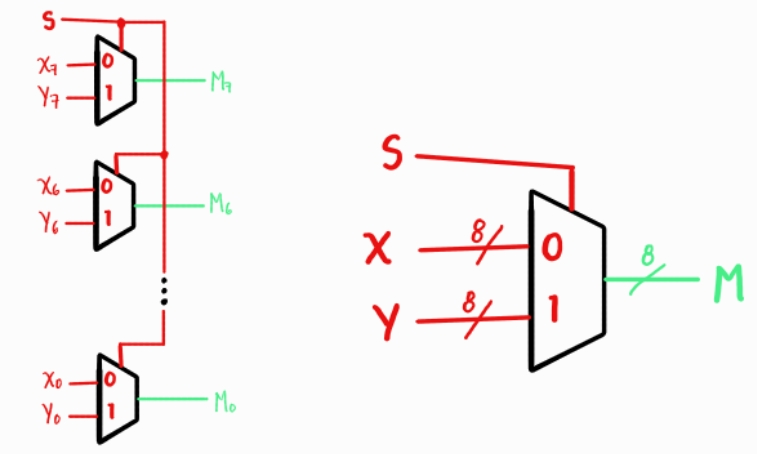
\includegraphics[width=0.55\textwidth]{figura2.jpg}
  \caption{Extensión del multiplexor a ocho bits.}
\end{figure}

\subsubsection{Descripción del programa}
El diseño se divide en dos módulos. El primero, \texttt{mux2a1.vhd}, describe el comportamiento del multiplexor de ocho bits. El segundo, \texttt{mux2a1\_8bits.vhd}, conecta el módulo con los interruptores y LEDs de la tarjeta.

\begin{lstlisting}[caption={Fragmento de la selección de un bit.}]
M(0) <= (NOT (S) AND X(0)) OR (S AND Y(0));
\end{lstlisting}

La misma expresión se aplica a las ocho posiciones del vector. En el módulo superior se conectan:
\begin{itemize}
  \item \(SW_{17}\): selector \(S\).
  \item \(SW_{7:0}\): entrada \(X\).
  \item \(SW_{15:8}\): entrada \(Y\).
  \item \(LEDR_{17:0}\): reflejo del estado de los interruptores.
  \item \(LEDG_{7:0}\): salida \(M\).
\end{itemize}

\begin{figure}[H]
  \centering
  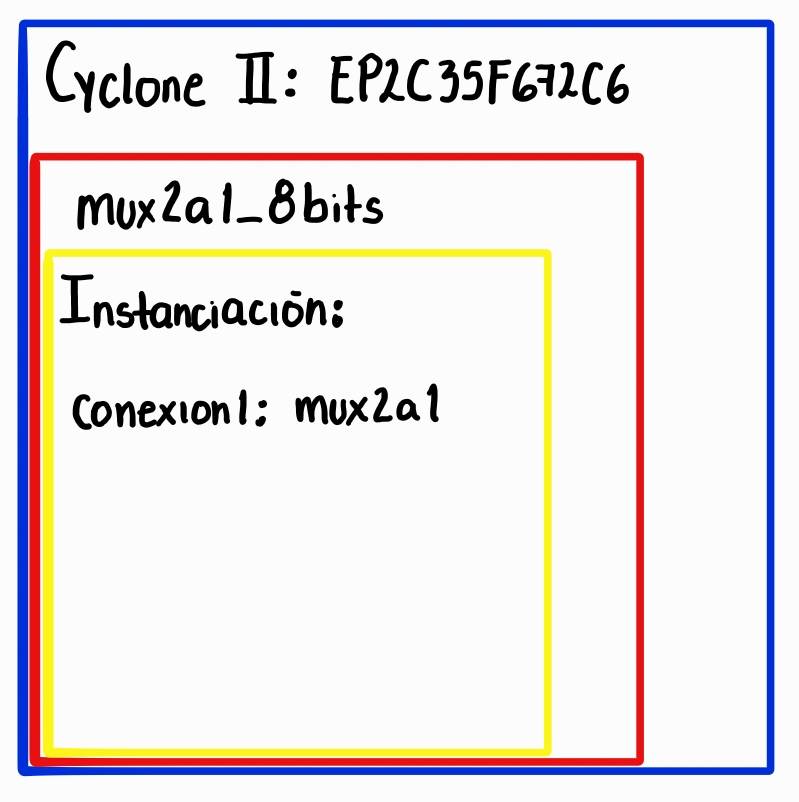
\includegraphics[width=0.55\textwidth]{figura3.jpg}
  \caption{Diagrama jerárquico del diseño de la Parte 2.}
\end{figure}

\subsubsection{Resultados y evidencia disponible}
En el material de la práctica se encuentra una captura del diagrama RTL generado después de la compilación y una captura de la simulación mediante un archivo de formas de onda.

\begin{figure}[H]
  \centering
  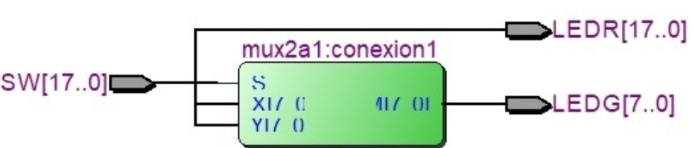
\includegraphics[width=0.78\textwidth]{figura4.jpg}
  \caption{Diagrama RTL de la Parte 2.}
\end{figure}

\begin{figure}[H]
  \centering
  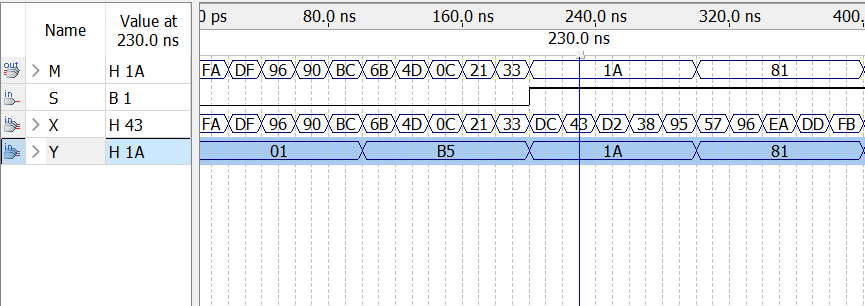
\includegraphics[width=0.78\textwidth]{figura5.png}
  \caption{Captura de la simulación de la Parte 2.}
\end{figure}

La descripción del reporte original indica que la simulación muestra la selección de \(X\) cuando \(S=0\) y de \(Y\) cuando \(S=1\). Estas capturas constituyen la evidencia visual disponible para esta parte.

\subsection{Parte 3. Multiplexor 5 a 1 de tres bits}

\subsubsection{Descripción del ejercicio}
Se describe un multiplexor de cinco entradas de un bit utilizando cuatro multiplexores 2 a 1. Posteriormente, el circuito se extiende a tres bits mediante tres instancias del módulo de un bit.

Las entradas de datos son \(U,V,W,X,Y\), y el selector está formado por \(S_2,S_1,S_0\). La estructura de selección implementada en el código corresponde a:

\[
M=
\begin{cases}
U, & S_2S_1S_0=000,\\
V, & S_2S_1S_0=001,\\
W, & S_2S_1S_0=010,\\
X, & S_2S_1S_0=011,\\
Y, & S_2=1.
\end{cases}
\]

Las combinaciones \(100\) a \(111\) seleccionan igualmente \(Y\), debido a la conexión del último multiplexor. Esta interpretación se obtiene de la estructura de instancias del archivo VHDL.

\subsubsection{Descripción del programa}
El diseño se organiza en tres niveles:
\begin{itemize}
  \item \texttt{mux2a1.vhd}: bloque básico de selección 2 a 1.
  \item \texttt{mux5a1.vhd}: combina cuatro bloques básicos para seleccionar una de cinco entradas.
  \item \texttt{mux5a1de3bits.vhd}: replica el multiplexor para cada posición de un vector de tres bits.
  \item \texttt{mux5a1\_3bits.vhd}: módulo superior que conecta los interruptores con las entradas y los LEDs verdes con la salida.
\end{itemize}

En el módulo superior, \(SW_{17:15}\) corresponde al selector y los quince interruptores restantes se distribuyen en grupos de tres bits para las entradas \(U,V,W,X,Y\). La salida se conecta a \(LEDG_{2:0}\), mientras que \(LEDR\) refleja los interruptores.

\subsubsection{Resultados y evidencia disponible}
Los archivos fuente VHDL permiten analizar la jerarquía y deducir la función de selección. Sin embargo, en las evidencias visuales disponibles en el repositorio no se identificó una captura específica del diagrama RTL ni de la simulación de esta parte. Por ello, no se afirma que exista una validación experimental documentada.

\subsection{Parte 4. Decodificador para display de siete segmentos}

\subsubsection{Descripción del ejercicio}
Se implementa un módulo decodificador que recibe un vector de tres bits y genera siete señales de salida, una para cada segmento del display. El diseño se divide en un módulo de comportamiento (\texttt{deco.vhd}) y un módulo de conexión (\texttt{decoder.vhd}).

\subsubsection{Descripción del programa}
El módulo \texttt{deco} recibe las señales \(C_2,C_1,C_0\) y produce las salidas \(a,b,c,d,e,f,g\). El módulo \texttt{decoder} recibe el vector de interruptores \(SW_{2:0}\), instancia el componente \texttt{deco} y conecta sus siete salidas con \(HEX0_{6:0}\).

Las expresiones booleanas encontradas en el archivo fuente son:

\begin{align*}
a &= C_2 \lor C_0,\\
b &= 1,\\
c &= C_2 \lor C_1 \lor C_0,\\
d &= C_2 \lor (\overline{C_1}\land C_0),\\
e &= C_2 \lor (\overline{C_1}\land\overline{C_0}),\\
f &= C_2,\\
g &= C_2 \lor (\overline{C_1}\land C_0).
\end{align*}

Estas expresiones se transcriben del código disponible. La correspondencia visual de los segmentos y la polaridad eléctrica del display deben verificarse con el instructivo de la tarjeta y con una prueba de hardware; no se infieren únicamente a partir de los nombres de las señales.

\subsubsection{Resultados y evidencia disponible}
Se encontró el código VHDL y el archivo de asignación de pines para \(SW_{2:0}\) y \(HEX0\). No se encontró una captura específica de simulación o de funcionamiento físico del decodificador, por lo que esta validación queda pendiente de documentar.

\subsection{Parte 5. Integración del multiplexor y el decodificador}

\subsubsection{Descripción del ejercicio}
Se integra el multiplexor de cinco entradas de tres bits con el decodificador de siete segmentos. El resultado de la selección se convierte en señales para un display. El módulo superior repite esta estructura para controlar cinco displays.

\subsubsection{Descripción del programa}
El archivo \texttt{muxdeco.vhd} instancia dos componentes:
\begin{itemize}
  \item \texttt{mux5a1de3bits}: selecciona una de las cinco entradas de tres bits.
  \item \texttt{decoder}: convierte el resultado seleccionado en siete señales de salida.
\end{itemize}

El módulo \texttt{parte5.vhd} distribuye las entradas entre cinco instancias de \texttt{muxdeco}. Cada instancia recibe el mismo selector \(SW_{17:15}\), pero cambia el orden de las entradas \(U,V,W,X,Y\). Las salidas se conectan a \(HEX0\), \(HEX1\), \(HEX2\), \(HEX3\) y \(HEX4\).

\subsubsection{Resultados y evidencia disponible}
Se localizaron los archivos VHDL de integración y un archivo de asignación de pines para los interruptores y los cinco displays. No se identificó evidencia visual de simulación o de prueba física correspondiente a esta integración. Por tanto, el funcionamiento descrito se presenta como análisis de la estructura del código y no como una comprobación experimental.

\section{Observaciones}
\begin{itemize}
  \item La organización jerárquica permite reutilizar módulos básicos para construir circuitos de mayor complejidad.
  \item La asignación de pines es parte necesaria de la implementación en la tarjeta DE2; los archivos de configuración disponibles contienen las correspondencias utilizadas.
  \item La evidencia visual localizada corresponde principalmente a la Parte 2. Para las Partes 3, 4 y 5 es necesario incorporar capturas de compilación, diagramas RTL, simulaciones o pruebas físicas.
  \item El archivo \texttt{PRACTICA-1/Parte6/parte6.vhd} está prácticamente vacío, por lo que no se incluye como ejercicio desarrollado.
  \item La polaridad y la interpretación visual del display deben confirmarse con el manual de la tarjeta y una prueba real.
\end{itemize}

\section{Conclusiones}
La práctica permite aplicar descripciones de hardware en VHDL mediante módulos combinacionales y conexiones jerárquicas. A partir del código disponible se identifica cómo un multiplexor elemental puede reutilizarse para construir selectores de mayor número de entradas y cómo su salida puede conectarse a un decodificador para controlar displays de siete segmentos.

La documentación disponible respalda con capturas la estructura RTL y la simulación de la Parte 2. Para considerar completas las demás validaciones es necesario agregar sus evidencias de compilación, simulación o funcionamiento en la tarjeta. De esta manera, se distingue entre el comportamiento deducido de los archivos fuente y los resultados efectivamente comprobados.

\end{document}
